% HELIOFLOOR -- independent evaluation of Surya's solar-flare head
% Draft v0.6. Compile: latexmk -pdf paper.tex
% Figures expected in figures/ as PDF (make_figures.py writes both PNG and PDF).
\documentclass[11pt]{article}

\usepackage[T1]{fontenc}
\usepackage[utf8]{inputenc}
\usepackage{lmodern}
\usepackage{microtype}      % even word spacing; also fixes extractor word-merging          % Unicode-mappable outlines
% Emit ToUnicode CMaps so copied and indexed text keeps fi/fl ligatures
% and Turkish characters. Without this, extraction turns flare into are.
\input{glyphtounicode}
\pdfgentounicode=1
\usepackage[margin=1in]{geometry}
\usepackage{graphicx}
\usepackage{booktabs}
\usepackage{amsmath}
\usepackage{amssymb}
\usepackage{textcomp}
\usepackage{url}
\usepackage[round,authoryear]{natbib}
\usepackage[hidelinks]{hyperref}
\usepackage{caption}

\graphicspath{{figures/}}
\captionsetup{font=small,labelfont=bf}

\newcommand{\Wm}{\,\mathrm{W\,m^{-2}}}
\newcommand{\code}[1]{\texttt{#1}}
\newcommand{\doi}[1]{doi:\href{https://doi.org/#1}{#1}}

\title{An Independent Evaluation of Surya's Solar Flare Forecasting:\\
Cheap Baselines Match a 366M-Parameter Foundation Model}

\author{Kadir Can Y\i{}ld\i{}r\i{}m\\[2pt]
\small Independent researcher, Eski\c{s}ehir, T\"urkiye\\
\small \texttt{kadir.can.yildirm@gmail.com} \,\textperiodcentered\,
ORCID: \href{https://orcid.org/0009-0008-5098-2547}{0009-0008-5098-2547}}
\date{Draft v0.6 --- \today}

\begin{document}
\maketitle

\begin{center}
\begin{minipage}{0.86\textwidth}
\small\textbf{Keywords:} solar flare forecasting, foundation models, benchmark
evaluation, model calibration, space weather, baseline comparison, base-rate
drift.
\end{minipage}
\end{center}
\vspace{6pt}

\begin{abstract}
Surya is a 366M-parameter heliophysics foundation model released by NASA and IBM,
pretrained on Solar Dynamics Observatory (SDO) imagery. Its accompanying paper
reports a solar flare forecasting result of TSS 0.436 (HSS 0.522, F1 0.561)
against two deep-learning image baselines. We present, to our knowledge, the first independent
evaluation of the released \code{solar\_flares\_surya} checkpoint. Streaming raw
SDO inputs from the official archive, we scored the model on 1{,}146 stratified
forecast hours spanning 2011--2024 (218 positive), and separately evaluated cheap
non-imagery baselines on the \emph{complete} official splits (3{,}672 validation
and 43{,}848 test hours).

We report five findings, ordered by the strength of their support.
(i) \textbf{The benchmark's effective sample is far smaller than it appears.}
Forecast hours inside a 24-hour block are strongly autocorrelated, so the unit of
evidence is the block, not the hour: our 739 validation hours occupy 50 blocks of
which only \textbf{6 contain any positive}, and 407 test hours occupy 28 blocks of
which 11 do. Block bootstrap accordingly yields 95\% intervals 0.46--0.81 TSS
wide; paired differences straddle zero for eight of ten method pairs, and
the strongest separation is the shipped 0.5 threshold scoring significantly
below 24-hour persistence on the test window ($\Delta$TSS $-0.445$, 95\% CI
$[-0.825, -0.086]$); no pair survives a ten-way family-wise correction, which
is the under-powering restated.
(ii) \textbf{Calibration is regime-dependent and does not transfer.} Surya's
probabilities are close to faithful on the validation window (Brier 0.057) and
collapse on the test window (Brier 0.208): across 15 independent blocks, hours
assigned 0.05--0.25 are followed by a flare 56.6\% of the time against a mean
predicted 0.148, and a Platt rescaling fitted on validation returns a
near-identity map that leaves decision quality unchanged.
(iii) \textbf{A cheap non-imagery baseline matches or exceeds the model.} An 11-feature logistic regression over the past week of GOES X-ray flux
---seconds to train on a CPU---ties Surya on identical validation hours (TSS
0.685 vs 0.673) and exceeds it on identical test hours (0.738 vs 0.632), a paired
difference that excludes zero, though only marginally; on the complete splits it reaches 0.661 and 0.554 against the reported 0.436, a
comparison we report but flag as unmatched.
(iv) \textbf{No trivial baseline is reported at all}: 24-hour persistence alone
reaches 0.430 on the full validation split, with a 95\% interval of
$[0.238, 0.621]$ that contains the reported 0.436.
(v) \textbf{Skill appears regime-split, but only its structural half is
estimable.} Persistence cannot anticipate a flare episode's onset by
construction, and false-alarms through every decay hour; the model's onset
behaviour, however, rests on just 4 and 3 independent onset-containing blocks and
therefore supports description but not estimation---we report it as an
observation, not a rate.

Findings (ii) and (v), together with the threshold behaviour in
Section~\ref{sec:baserate}, share one mechanism: base-rate non-stationarity. The
positive rate in the official test split rises from 0.0055 in 2020 to 0.697 in
2024, a 128-fold shift across the solar cycle. Under a frozen threshold the two cheap
methods move in opposite directions, yet the pooled test TSS exceeds every
per-year value for both, a textbook Simpson's paradox. Finding (i) has a separate cause, the
combination of temporal autocorrelation with event rarity, and finding (iii) a
third, the information already carried by the X-ray record.

Independently of our measurements, we document that the reported 0.436 cannot be
located: the released artifacts give three mutually incompatible split
definitions and the results table names none of them, while the two companion
papers report ResNet50 at TSS 0.018 and 0.261 for the same task, a reference
level less stable than the margin being claimed.

We therefore argue that the deficiency is not specific to Surya but structural to
the evaluation protocol, and we propose concrete fixes: mandatory cheap
baselines, per-regime rather than pooled reporting, explicit threshold
procedures, and uncertainty intervals computed over temporal blocks.
\end{abstract}

\section{Introduction}

Foundation models have begun to arrive in the physical sciences, and heliophysics
is among the newest arrivals. Surya, released in August 2025 by NASA and IBM
\citep{roy2025}, is a 366M-parameter transformer pretrained on Solar Dynamics
Observatory imagery and published openly with adapted heads for several
downstream tasks. Its release was accompanied by SuryaBench \citep{roy2026}, a
benchmark suite whose solar flare forecasting task asks a deceptively simple
question: given full-disk solar imagery at time $t$, will the peak GOES soft
X-ray flux exceed M1.0 during the next 24 hours?

Benchmarks of this kind do more than measure models; they define what the field
will treat as progress. A reported score becomes the number that later work must
beat, the number that funding proposals cite, and the number that operational
users read as an indication of readiness. That gives the \emph{design} of the
evaluation---which baselines appear, how the score is aggregated, whether
uncertainty is quoted---at least as much influence on the field as the model
itself.

Independent evaluation of such models is nevertheless rare, for a mundane reason:
it is expensive. Each forecast hour in this task requires two SDO timesteps of 13
channels at $4096^2$ resolution; scoring even a modest sample means streaming
hundreds of gigabytes through a GPU. The practical consequence is that reported
numbers tend to go unchallenged, not because they are beyond challenge but
because checking them costs more than most groups will spend.

This paper reports what we found when we paid that cost. We evaluated the
released \code{solar\_flares\_surya} checkpoint with the authors' own inference
code on 1{,}146 stratified forecast hours spanning 2011--2024, and---because they
require no GPU at all---we evaluated cheap non-imagery baselines on the complete
official splits, 3{,}672 validation and 43{,}848 test hours. To our knowledge,
no independent evaluation of the released checkpoint has been reported.

Our contributions are six. The first five are measurements, and they compound;
the sixth is documentary and independent of anything we ran.

\begin{enumerate}
\item \textbf{The benchmark reports no cheap baseline.} Its comparators are two
image models (AlexNet, ResNet50). A 24-hour persistence rule, which requires no
model at all, already reaches TSS 0.430 on the full validation split, with a
day-blocked 95\% interval of $[0.238, 0.621]$ that contains the 0.436 reported
for the foundation model.
\item \textbf{A cheap non-imagery model matches or exceeds the foundation
model.} On the \emph{same} forecast hours, an 11-feature logistic regression over
the past week of GOES X-ray flux ties Surya on validation (0.685 vs 0.673) and
beats it on test (0.738 vs 0.632). On the complete splits it reaches 0.661 and
0.554, above the reported 0.436, a comparison we report but flag as unmatched,
since full-split inference of the model was beyond our compute budget.
\item \textbf{Single-number comparisons on this task are under-powered.}
Forecast hours within a 24-hour block are strongly autocorrelated; resampling
whole blocks yields 95\% intervals 0.46--0.81 TSS wide; paired block-bootstrap differences
straddle zero for eight of ten method pairs, and even the strongest
separation---the shipped threshold falling below persistence on test---does
not survive a ten-way family-wise correction.
\item \textbf{Skill appears regime-split, and the two regimes are
complementary.} Persistence is structurally blind to episode onsets and
false-alarms on every decay hour, a definitional statement that holds at any
sample size. The model's complementary behaviour on onsets is visible in our
sample but, as Section~\ref{sec:onset} shows, rests on too few independent
episodes to be quoted as a rate.
\item \textbf{Calibration is regime-dependent and does not transfer.} Surya's
probabilities are close to faithful in the validation window and collapse in the
test window; a rescaling fitted on the former transfers as a near-identity map
and changes nothing.
\item \textbf{The reported score cannot be located in the released artifacts.}
Three incompatible split definitions are on offer and the results table names
none of them; the two companion papers disagree by a factor of fourteen on the
same baseline's TSS; and the dataset documentation states an event threshold one
order of magnitude away from the one its own labels follow. This is a reading of
the public record, not a measurement, and it is set out with sources in
Section~\ref{sec:located}.
\end{enumerate}

Contributions 4 and 5, and the threshold behaviour documented in
Section~\ref{sec:baserate}, share one cause. The positive rate in the official
test split rises from 0.0055 in 2020 to 0.697 in 2024 as the solar cycle climbs
toward maximum, a 128-fold shift within a single split. Under a frozen decision
threshold the cheap methods move in opposite directions, and pooling across the
split produces, for each of them, a score higher than that of any individual
year. Contribution 3 has a different
origin---autocorrelation and event rarity, and contribution 2 a third, namely
how much of the 24-hour flare signal the X-ray record already carries.

We therefore frame this work as a critique of an evaluation protocol rather than
of a model. The authors themselves describe the downstream heads as
``proof-of-concept studies \ldots{} not optimized for end-to-end or operational
forecasting use,'' and we take that qualification at face value. Our claim is
narrower: \emph{even as a proof of concept, this protocol cannot rank methods}, because the contribution of the imagery modality
is never isolated from what X-ray history alone provides. We close with six
concrete changes that would restore that ability, all of them cheap.

\section{Background}

\subsection{Surya and SuryaBench}

Surya is a 366M-parameter transformer over 13 SDO channels---8 AIA (seven EUV
plus one UV at 1600\,\AA) and 5 HMI (line-of-sight magnetic field, three vector
components, Doppler velocity)---at $4096^2$ native resolution, released on
Hugging Face under Apache 2.0 with LoRA-adapted downstream heads.

We are deliberately careful about the size of the pretraining corpus, because the
released artifacts do not agree. The model paper states that the ML-ready SDO
database spans ``May 13, 2010, to December 31, 2024'' and that ``the total size of
the data for dataset is around 257 TB'' (its Section 2.1.2), and separately that
the pretraining partition used ``observations from 2011 to 2019.'' The Hugging
Face model card instead describes the model as ``pretrained on 9 years
($\approx$218 TB) of multi-instrument data.'' The strings ``218'' and ``nine
years'' do not appear in the paper. No released source states how the two
relate: the paper never gives 218 TB, the model card never gives 257 TB, and
neither connects a nine-year pretraining corpus to the full 2010--2024 database.
We cite the 218 TB to the model card, its only source, and leave the two figures
unreconciled rather than reconciling them on the authors' behalf. This is a small illustration of a pattern documented
in Section~\ref{sec:located}.

\subsection{The flare forecasting task}

Binary: does the peak GOES soft X-ray flux exceed
$\theta_{\max} = 10^{-5}\Wm$ (M1.0) in the window $[t, t+24\mathrm{h})$? Hourly
cadence. Model input is two timesteps ($t-60$\,min and $t$). The official splits,
as they appear in the released CSVs, are given in Table~\ref{tab:splits}.

\begin{table}[htbp]
\centering
\caption{The official splits as they exist in the released files, counted
directly. The dataset card describes validation and \code{leaky\_validation} as
covering 2010--2019, but 2010 is absent from both
($3{,}672 = 17\ \mathrm{days} \times 24\,\mathrm{h} \times 9\ \mathrm{years}$).}
\label{tab:splits}
\begin{tabular}{lllrr}
\toprule
split & years & calendar window & hours & base rate \\
\midrule
train & 2010--2019 & Feb 15 -- Dec 31 & 74{,}760 & 0.1211 \\
validation & 2011--2019 & Jan 15--31 & 3{,}672 & 0.1089 \\
\code{leaky\_validation} & 2011--2019 & Jan 1--14, Feb 1--14 & 6{,}048 & 0.1490 \\
test & 2020--2024 & full year & 43{,}848 & 0.2943 \\
\bottomrule
\end{tabular}
\end{table}

Two features of this design matter later. The validation split is a set of
seventeen-day January windows drawn from the \emph{same} years as training, which
the authors implicitly acknowledge by naming the adjacent split
\code{leaky\_validation}. And the test split spans the rising phase of solar
cycle 25, so its base rate is not stationary (Section~\ref{sec:baserate}).

\subsection{Reported results and why they cannot be located}
\label{sec:located}

Table 4 of the model paper reports Surya at TSS 0.436 / HSS 0.522 / F1 0.561
against AlexNet (0.358 / 0.398 / 0.454) and ResNet50 (0.018 / 0.028 / 0.055).
Both comparators are image models. \textbf{The evaluation split is not stated;
the decision-threshold procedure is not stated; no uncertainty is reported; no
non-imagery baseline appears.} We read that section in full: it defines the
label, then the metrics, then presents the table. There is no
train/validation/test partition for this task, no date range, no sample count,
and no description of how a probability is converted into a binary forecast.

This is worse than an omission, because the released artifacts offer three
\emph{mutually incompatible} candidates for the missing split
(Table~\ref{tab:threesplits}).

\begin{table}[htbp]
\centering
\caption{Three incompatible candidate splits, none of which the results table
names.}
\label{tab:threesplits}
\small
\begin{tabular}{llll}
\toprule
source & training & validation & test \\
\midrule
model paper, SDO-data section & 2011--2019, days 46--365 & --- & 2011--2019, days 15--31 \\
SuryaBench, core SDO data & 2010--2018 & 2019 & 2020 \\
Hugging Face flare dataset card & 2010--2019, Feb 15--Dec 31 & Jan 15--31 & 2020--2024 \\
\bottomrule
\end{tabular}
\end{table}

The model paper's partition is given in the SDO-data section and never linked to
the downstream tasks; the SuryaBench figure is for the core dataset, with file
counts ($379{,}920 / 43{,}680 / 43{,}800$) that do not correspond to the hourly
flare task at all. Since the results table names none of them, \textbf{TSS 0.436
is not attributable to any specific evaluation period.} Our own reading---that it
most plausibly refers to the Jan 15--31 validation window---is an inference, and
we mark it as one wherever it matters.

A second discrepancy is sharper still. The two companion papers, submitted the
same day by overlapping author lists, report irreconcilable numbers for the same
baseline architectures on the same task:

\begin{table}[htbp]
\centering
\caption{The same baselines, the same task, two companion papers.}
\label{tab:baselinegap}
\begin{tabular}{lll}
\toprule
model & Surya paper, Table 4 & SuryaBench, Table 3(b) \\
\midrule
AlexNet & TSS 0.358, HSS 0.398, F1 0.454 & TSS 0.359, HSS 0.354, F1 0.679 \\
ResNet50 & TSS \textbf{0.018}, HSS 0.028, F1 0.055 & TSS \textbf{0.261}, HSS 0.281, F1 0.627 \\
\bottomrule
\end{tabular}
\end{table}

In Table~\ref{tab:baselinegap}, ResNet50's TSS differs by a factor of about
fourteen and AlexNet's F1 by 0.225.
Which is right we cannot say, and that is what matters here: the reference level
against which the foundation model's 0.436 is judged is itself unstable by more
than the margin being claimed. Whatever explains the gap---a different split, a different
threshold, a different training run---is exactly the information neither table
records.

We note one further inconsistency because it affects anyone reproducing the task.
The SuryaBench text says its binary thresholds correspond ``to the equivalent
strength of an M1.0-class flare'' while stating the threshold as $10^{-4}\Wm$,
which is X1.0, not M1.0. The model paper uses $10^{-5}\Wm$ (M1.0). We resolved
the ambiguity empirically against the released labels themselves: they follow
M1.0, as verified on all 128{,}328 rows in Section~\ref{sec:leak}.

\subsection{A label-leakage trap in the released data}
\label{sec:leak}

In the released flare CSVs, \code{max\_goes\_class[t]} is the maximum class over
$[t, t+24\mathrm{h})$---i.e.\ it is the source of the label, not a past
observation. We verified
$\code{label\_max} == (\code{max\_goes\_class} \geq \mathrm{M1.0})$
on 128{,}328 of 128{,}328 rows. Any baseline that reads this column at time $t$
is therefore trivially perfect and meaningless. The same holds for
\code{cumulative\_index}: the dataset card defines it over the same prediction
window, and we verified the exact identity
$\code{label\_cum} == (\code{cumulative\_index} \geq 10)$ on 128{,}328 of
128{,}328 rows. All features in this work are read at $t-24$h or earlier; at
that lag both forward-looking columns cover $[t-24\mathrm{h}, t)$ and are
legitimately observable at forecast time.

\subsection{Related work: a standard practice this benchmark omits}

Solar flare forecasting already has a community standard for comparative
evaluation. \citet{barnes2016}, reporting the 2009 interagency ``all-clear''
workshop in Boulder, established the methodology and concluded that ``there is no
single method that is clearly better than the others for flare prediction in
general,'' with no participating method proving substantially better than
climatology. The follow-on series---\citet{leka2019b},
\citet{leka2019c} and \citet{park2020}---arose from a separate 2017 meeting at
the Institute for Space-Earth Environmental Research, Nagoya University, and
applied the methodology to operational forecasting systems worldwide. Its central
conclusion is directly relevant here. In the words of Paper II's abstract:

\begin{quote}
``Numerous methods performed consistently above the `no skill' level, although
which method scored top marks is decisively a function of flare event definition
and the metric used; there was no single winner.''
\end{quote}

That series also normalised reporting climatological reference levels and
examining metric sensitivity rather than quoting one number.

We therefore make no claim to have discovered that simple methods are
competitive; that result is nearly a decade old, and our
Section~\ref{sec:cheap} is a re-demonstration of it in a new setting. Our
contribution is the observation that a prominently released 2025
foundation-model benchmark \textbf{departs from these established practices}: it
reports a single pooled TSS against two image models, without a non-imagery or
climatological reference, without stating the evaluation split or the threshold
procedure, and without uncertainty. Read against \citet{barnes2016} and the
Leka/Park series, the reported comparison cannot support a ranking claim---and
our measurements show concretely what that omission conceals: metric-dependent
ordering (Section~\ref{sec:cheap}), interval overlap
(Section~\ref{sec:power}), regime-split skill (Section~\ref{sec:onset}), and
non-transferable calibration (Section~\ref{sec:calib}).

\subsection{Reference forecasts in research and in operations}

Comparison against explicit reference forecasts is not a preference of ours; it
is what this field already does, and the operational agency applies it to its own
product. NOAA's Space Weather Prediction Center issues daily probabilistic M- and
X-class flare forecasts---percentages from 1\% to 99\% for a specified 24-hour
day, at lead times of one to three days, and its published verification measures
their skill \emph{against short-term (30-day) climatology and 1-day persistence},
defining negative skill as no improvement over a constant climatological forecast
\citep{swpcverif}. The same expectation runs through the research literature:
\citet{leka2019b} argue that in operational settings the appropriate standard is
``the best `unskilled' forecast available,'' and the TSS itself---the
Hanssen--Kuipers discriminant, or Peirce skill score---was adopted as the standard
flare metric precisely to make cross-method comparison meaningful
\citep{bloomfield2012}.

Two recent results make the omission we document harder to excuse. First, in the
SHARP-parameter tradition \citep{bobra2014} that has dominated machine-learning
flare forecasting since \citet{bobra2015}---who report a TSS of 0.76 in their
operational configuration for $\geq$M1.0 within 24 hours---feature-ranking studies
repeatedly find prior flare activity among the strongest individual predictors
\citep{nishizuka2017,campi2019}, and \citet{vandersande2023}, forecasting M-class
flares at 24 hours from magnetogram data, conclude that ``flaring history has
greater predictive power than our CNN-extracted features.'' Our
Section~\ref{sec:cheap} is that finding again, against a much larger image model.
Second, and most directly, \citet{camporeale2025} verified 27 years of SWPC flare
forecasts and report that ``even the simple persistence model---using no training
and based solely on the previous day's flare activity---performs on par with, or
only marginally below, the SWPC forecast.'' They close with a recommendation we
would have been happy to write ourselves:

\begin{quote}
``Any solar flare forecasting or all-clear prediction models developed in a
research setting should perform the type of basic forecast verification study
shown here --- using the same baseline models and metrics for comparison ---
before being claimed as an advance over current methods.''
\end{quote}

That was published in \emph{Space Weather} in the same year as the model we
evaluate. Our contribution is not the idea of checking against persistence; it is
that nobody had checked \emph{this} model, and that the benchmark as published
does not let a reader do so.

We do not overstate the SHARP literature. We did not find a study
that pits a flare-history-only model directly against a SHARP-parameter model at
equal footing with both scores reported, and we do not claim one exists;
\citet{vandersande2023} is the closest, and it compares flare history against
CNN-extracted magnetogram features rather than SHARP scalars. Nor did we run a
SHARP baseline ourselves (Section~\ref{sec:limits}).

\section{Methods}

\subsection{Model evaluation}

Released checkpoint \code{nasa-ibm-ai4science/solar\_flares\_surya} with the
authors' own \code{infer.py}, \code{SolarFlareDataset}, \code{config\_infer.yaml}
and scalers; raw netCDF inputs streamed from the official S3 archive (download
$\rightarrow$ infer $\rightarrow$ delete). bf16 autocast on a T4. Deterministic:
seed 42, no shuffling, no augmentation. Every label we scored was re-checked
against the official split CSVs: 0 mismatches on 739 validation and 407 test
hours. Pinned revisions: checkpoint \code{ec7c42a} (2025-08-18), flare dataset
\code{bf474bc} (2025-12-16; a comparison of the label files shows that revision
touched only the dataset README).

\subsection{Sampling}
\label{sec:sampling}

Full-split inference is prohibitive. Each forecast hour needs two timesteps at
$\sim$586\,MB each, and consecutive hours within a block share one of them;
scoring our sample required 1{,}224 distinct netCDF files, roughly 700\,GB
streamed. Covering the full test split alone would have required about 25\,TB.

We therefore drew a seeded, stratified sample of contiguous 24-hour windows---36
validation windows (2011--2019) and 20 test windows (2020--2024)---deliberately
over-sampling flare-active periods so that positives are sufficiently
represented. Missing archive files cost 125 of the 864 planned validation hours
and 73 of the 480 planned test hours, about 15\% in each case, and those gaps
fragment some windows: the 36 planned validation windows survive as 50 contiguous
runs (20 of at least 20 hours, 30 shorter fragments), and the 20 planned test
windows as 28 runs (14 of at least 20 hours). Throughout this paper a
\emph{block} means one of these recovered contiguous runs, since that is the unit
within which hours are actually autocorrelated.

The resulting sample base rates (0.115 validation, 0.327 test) are higher than the
full-split rates; absolute values are therefore not directly comparable to
full-split numbers, but every model comparison is made on identical hours.

\paragraph{Sampling sanity check.} Because the cheap baselines need no GPU we
could score them both on our sample and on the complete splits. Estimates agree
closely (GOES logistic 0.685 vs 0.661; persistence 0.405 vs 0.430), indicating
that the stratification does not materially distort model ranking.

\subsection{Baselines}

\begin{enumerate}
\item \textbf{Climatology}---always predict ``no flare''.
\item \textbf{Persistence}---predict the label observed at $t-24$h, read from the
complete hourly record rather than from the split file, so that no hour is
dropped merely because its reference falls in a neighbouring split.
\item \textbf{GOES-history logistic regression}---11 features from lags $t-24$h
\ldots{} $t-168$h (log peak flux per lag, 7-day max, cumulative-index terms),
standardised, L2-regularised, fitted by gradient descent on the official train
split (74{,}564 of 74{,}760 rows; 196 dropped for non-finite features, see
Section~\ref{sec:limits}). Trains in seconds on a CPU.
\end{enumerate}

\subsection{Metrics and uncertainty}

TSS (POD $-$ POFD), HSS, F1, full confusion matrices, and a full threshold sweep.
Hourly samples within a 24-hour block are strongly autocorrelated, so naive
per-sample bootstrap understates variance; we resample \textbf{whole blocks} (50
validation, 28 test for the sampled hours; calendar days for the complete splits)
and report percentile 95\% intervals. Each interval reseeds its own generator, so
a printed interval reproduces on its own rather than depending on how many
intervals were drawn before it.

\section{Results}

\subsection{The missing baseline}

On the full validation split, persistence alone reaches TSS 0.430 with a
day-blocked 95\% interval of $\mathbf{[0.238, 0.621]}$, an interval that
contains the 0.436 reported for a 366M-parameter model. Because no uncertainty is reported
alongside the 0.436, the two numbers cannot be formally compared. What the
interval does show is that the sampling variability of the \emph{trivial}
baseline alone covers the reported result, the information a benchmark table
should make visible, and this one does not. On the full test split persistence reaches
0.535 $[0.502, 0.568]$.

\subsection{A cheap non-imagery model matches or exceeds the foundation model}
\label{sec:cheap}

\paragraph{Matched comparison (identical hours, our measurements only).} This is
the primary result because both numbers come from the same forecast hours.

\begin{table}[htbp]
\centering
\caption{Matched comparison on identical forecast hours.}
\begin{tabular}{lrrrr}
\toprule
split & hours & GOES-history logistic & Surya (tuned) & Surya @0.5 \\
\midrule
validation & 739 & \textbf{0.685} & 0.673 & 0.425 \\
test & 407 & \textbf{0.738} & 0.632 & 0.173 \\
\bottomrule
\end{tabular}
\end{table}

On validation the two are indistinguishable; on test the cheap model leads on
every metric (HSS 0.699 vs 0.571, F1 0.807 vs 0.735), and the paired
block-bootstrap TSS difference excludes zero, though only marginally ($+0.106$,
95\% CI $[+0.009, +0.280]$; Section~\ref{sec:power}). Both thresholds are tuned
in-sample, which flatters both equally.

\paragraph{Unmatched comparison (full splits, reported number).} Because the
baselines need no GPU we could also score them on every official hour, with a
no-cherry-picking protocol: weights from the train split, a single threshold
chosen on the full validation split (0.10) and frozen for test.

\begin{table}[htbp]
\centering
\caption{Complete official splits under a frozen-threshold protocol. Intervals
are day-blocked bootstrap.}
\begin{tabular}{lrrlrlrr}
\toprule
split & $n$ & base & model & TSS & 95\% CI & HSS & F1 \\
\midrule
validation (full) & 3{,}672 & 0.109 & GOES logistic & \textbf{0.661} & $[0.532, 0.777]$ & 0.375 & 0.475 \\
validation (full) & 3{,}672 & 0.109 & persistence & 0.430 & $[0.238, 0.621]$ & 0.428 & 0.491 \\
test (full) & 43{,}848 & 0.294 & GOES logistic & \textbf{0.554} & $[0.526, 0.581]$ & 0.436 & 0.655 \\
test (full) & 43{,}848 & 0.294 & persistence & 0.535 & $[0.502, 0.568]$ & 0.536 & 0.672 \\
\bottomrule
\end{tabular}
\end{table}

Because Section~\ref{sec:located} leaves three candidate readings of the reported
split, we checked the cheap baseline against all three. Under the model paper's
partition (days 15--31 of 2011--2019, i.e.\ exactly the validation split) it
scores 0.661; under the dataset card's (2020--2024) it scores 0.554; under
SuryaBench's (2020 alone) it scores 0.452 (Section~\ref{sec:baserate}). Every one
exceeds 0.436, so the comparison does not depend on resolving the ambiguity---and
on validation the cheap model's own interval excludes the reported value.
\textbf{We flag this comparison as unmatched:} the baseline was run on all hours,
the model on our sample, and the 0.436 is the authors' own measurement rather
than ours. It is offered as corroboration of the matched result above, not as the
primary claim. The day-blocked intervals are also robust to the blocking unit:
with 2-day and 3-day blocks the validation persistence interval still contains
0.436 and the validation GOES interval still excludes it
(\code{gaps\_audit.py}).

\paragraph{The advantage is metric-dependent.} Against the
\emph{full validation split}, the reported HSS (0.522) and F1 (0.561) exceed the
cheap baseline's 0.375 and 0.475, the baseline buys its TSS with a high
false-alarm rate (740 false alarms against 355 hits). We therefore do not claim
uniform superiority; we claim that on TSS, the base-rate-independent metric
standard in this literature, the imagery modality shows no measurable advantage
over X-ray history on this task. On the matched test hours the cheap model does
lead on all three metrics simultaneously.

\subsection{Single-number comparisons are under-powered}
\label{sec:power}

\begin{table}[htbp]
\centering
\caption{Block-bootstrap intervals on our measured hours.}
\begin{tabular}{llrlr}
\toprule
split & model & TSS & 95\% CI & width \\
\midrule
validation & Surya @0.5 & 0.425 & $[0.028, 0.746]$ & 0.72 \\
validation & Surya @0.16 (tuned) & 0.673 & $[0.289, 0.886]$ & 0.60 \\
validation & persistence & 0.405 & $[-0.019, 0.792]$ & 0.81 \\
validation & GOES logistic @0.10 & 0.685 & $[0.417, 0.881]$ & 0.46 \\
test & Surya @0.5 & 0.173 & $[0.000, 0.484]$ & 0.48 \\
test & Surya @0.04 (tuned) & 0.632 & $[0.315, 0.876]$ & 0.56 \\
test & persistence & 0.618 & $[0.258, 0.889]$ & 0.63 \\
test & GOES logistic @0.34 & 0.738 & $[0.467, 0.940]$ & 0.47 \\
\bottomrule
\end{tabular}
\end{table}

Intervals are 0.46--0.81 TSS wide. Overlap between individual intervals is,
however, weak evidence about a difference; the same resampled blocks move both
scores together, so we resample pairs as well: one block draw per iteration
scores every method, and the interval of the paired difference is what decides
separation (\code{paired\_diff.py}; 4{,}000 draws; thresholds fixed at their
full-sample values).

\begin{table}[htbp]
\centering
\caption{Paired block-bootstrap differences in TSS. Bold rows exclude zero.}
\begin{tabular}{llrl}
\toprule
split & paired difference & $\Delta$TSS & 95\% CI \\
\midrule
validation & GOES logistic $-$ Surya (tuned) & $+0.012$ & $[-0.325, +0.473]$ \\
validation & Surya (tuned) $-$ persistence & $+0.268$ & $[-0.153, +0.658]$ \\
validation & GOES logistic $-$ persistence & $+0.279$ & $[-0.058, +0.681]$ \\
validation & Surya @0.5 $-$ persistence & $+0.019$ & $[-0.398, +0.427]$ \\
test & GOES logistic $-$ Surya (tuned) & $\mathbf{+0.106}$ & $\mathbf{[+0.009, +0.280]}$ \\
test & Surya (tuned) $-$ persistence & $+0.014$ & $[-0.210, +0.253]$ \\
test & GOES logistic $-$ persistence & $+0.120$ & $[-0.009, +0.330]$ \\
test & Surya @0.5 $-$ persistence & $\mathbf{-0.445}$ & $\mathbf{[-0.825, -0.086]}$ \\
\bottomrule
\end{tabular}
\end{table}

Eight of ten paired differences straddle zero (the two hybrid pairs,
Section~\ref{sec:onset}, also straddle). The two that do not are instructive.
The cheap baseline's advantage over tuned Surya on the test hours excludes zero
only marginally (lower bound $+0.009$), and we read it as suggestive rather than
decisive. The strongest separation in the study is negative:
\textbf{at its shipped 0.5 threshold the model scores significantly below
24-hour persistence on the test window} ($-0.445$, $[-0.825, -0.086]$).

Both exclusions, however, are made at the conventional 95\% level while ten
comparisons run simultaneously, and neither survives that accounting: the
bootstrap tail fractions are 0.55\% and 0.70\% against the 0.25\% a ten-way
Bonferroni correction demands, and the corrected 99.5\% intervals reach zero
($[0.000, +0.382]$) or cross it ($[-0.924, +0.070]$) (\code{gaps\_audit.py}).
We therefore describe the shipped-threshold deficit as the strongest separation
in the study rather than an unconditional one, and note that even our clearest
gap failing a family-wise correction is finding (i) restated: at 50 and 28
blocks, this protocol resolves almost nothing.

The reason differences this large are needed is visible once blocks are counted
rather than hours: of 50
validation blocks only \textbf{6 contain any positive}, and of 28 test blocks
only 11 do. Since the hit-rate term of TSS is determined entirely by
positive-containing blocks, the effective sample behind every published
flare-forecasting TSS is far smaller than the quoted hour count suggests.
\textbf{We recommend that the number of positive-containing independent blocks be
reported alongside any such score}; it is a one-line addition that would prevent
most over-reading.

\begin{figure}[htbp]
\centering
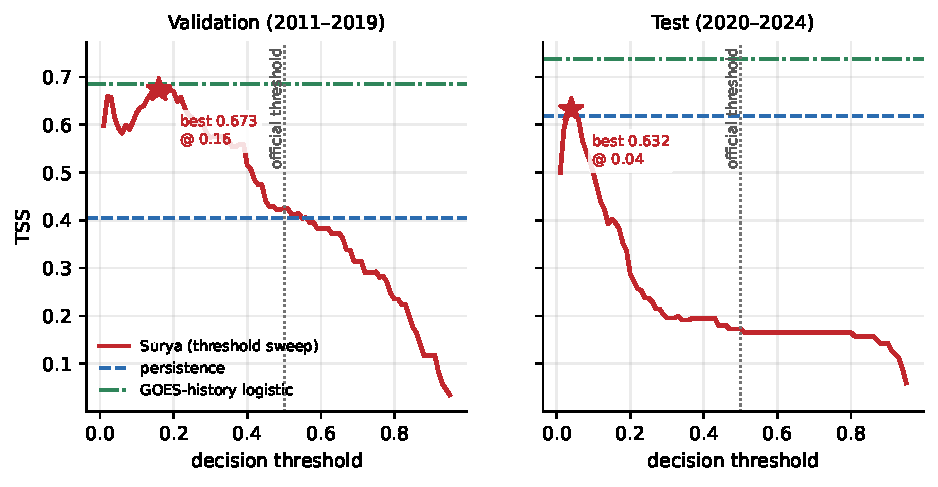
\includegraphics[width=\textwidth]{fig3_threshold_sweep}
\caption{TSS as a function of the decision threshold, with the two cheap
baselines as reference lines. The shipped 0.5 threshold sits far from any
optimum in both windows.}
\end{figure}

\subsection{Skill appears regime-split, and a trivial hybrid wins}
\label{sec:onset}

\begin{table}[htbp]
\centering
\caption{Positives partitioned by the persistence reference.}
\begin{tabular}{lrr}
\toprule
 & validation & test \\
\midrule
onset positives (persistence blind) & 46 & 27 \\
continuation positives & 39 & 106 \\
decay hours (persistence false-alarms) & 35 & 49 \\
onsets caught --- persistence & 0/46 & 0/27 \\
onsets caught --- Surya (tuned) & 35/46 & 13/27 \\
onsets caught --- Surya @0.5 & 14/46 & 0/27 \\
decay false alarms --- persistence & 35/35 & 49/49 \\
decay false alarms --- Surya (tuned) & 10/35 & 38/49 \\
\bottomrule
\end{tabular}
\end{table}

The two columns differ in kind. The persistence column is not a
statistical result: a rule that copies the label from $t-24$h cannot flag an
episode that had not yet begun, and must flag every hour of a decaying one. Those
entries are definitional and hold at any sample size.

The model's onset behaviour is a different matter, and its limits are severe. The 46 validation and 27 test onset hours occupy only \textbf{4 and 3
independent blocks} respectively, a handful of flare episodes, not a sample of
onsets. Block-bootstrap intervals for the catch rate are correspondingly useless.

\begin{table}[htbp]
\centering
\caption{Onset catch rates. Only the tuned rows carry information, and barely.}
\begin{tabular}{lllrlc}
\toprule
split & predictor & caught & rate & 95\% CI & blocks with a hit \\
\midrule
validation & Surya @0.16 (tuned) & 35/46 & 0.761 & $[0.357, 1.000]$ & 4/4 \\
validation & Surya @0.50 (shipped) & 14/46 & 0.304 & $[0.000, 0.750]$ & 3/4 \\
test & Surya @0.04 (tuned) & 13/27 & 0.481 & $[0.000, 1.000]$ & 2/3 \\
test & Surya @0.50 (shipped) & 0/27 & 0.000 & $[0.000, 0.000]$ & 0/3 \\
\bottomrule
\end{tabular}
\end{table}

The last row invites a misreading. A bootstrap interval of $[0.000, 0.000]$ around a 0/27 observation is a
boundary artefact of resampling a sample that contains no successes, not evidence
of precision. For a zero count the appropriate one-sided statement is the rule of
three applied to the \emph{effective} sample: with three onset-containing blocks
the 95\% upper bound is $3/3 \approx 1.0$, which constrains nothing at all.

We therefore report the onset results as \textbf{descriptive observations on a
handful of flare episodes, not as rate estimates}: in the three test episodes
sampled, the model at its shipped threshold flagged none of the 27 constituent
hours, and at a tuned threshold flagged hours in two of the three. The observation is striking and worth
checking at scale, but it is not a measured miss rate. The same caution applies to the
validation column, where the tuned threshold flags hours in all four episodes.

The two predictors are nonetheless complementary rather than competing, and that
statement rests on the pooled score rather than on the onset counts:
\emph{persistence OR Surya} reaches TSS 0.705 on validation, above either
component (0.673 / 0.405), a point-estimate ordering; the paired difference
against the stronger component straddles zero ($+0.032$, $[-0.044, +0.241]$).

\begin{figure}[htbp]
\centering
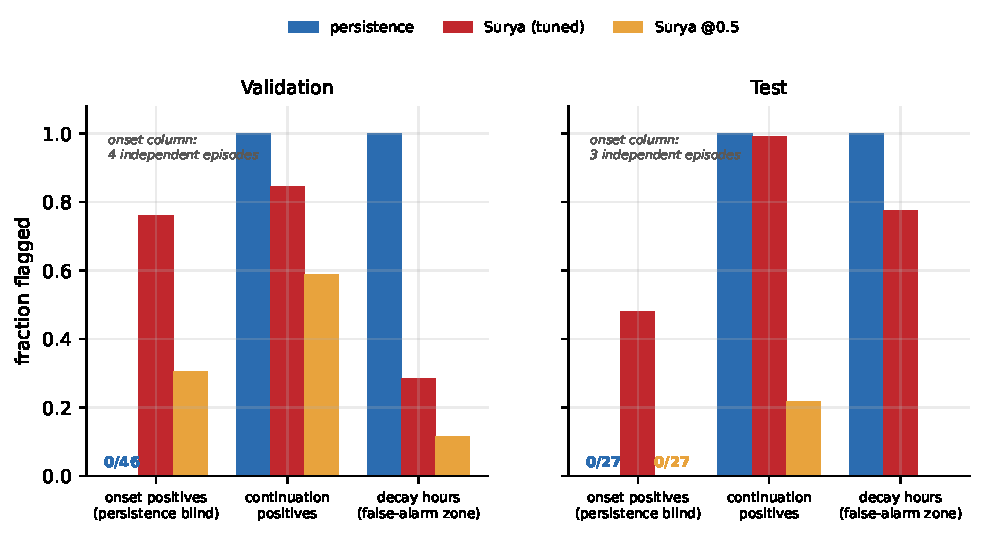
\includegraphics[width=\textwidth]{fig4_onset_continuation}
\caption{Complementary skill by regime. Persistence is structurally blind to
onsets and false-alarms through every decay hour. The onset column rests on four
(validation) and three (test) independent episodes and is descriptive only.}
\end{figure}

\subsection{Calibration is regime-dependent and does not transfer}
\label{sec:calib}

\begin{table}[htbp]
\centering
\caption{Complete reliability tables, with the number of independent blocks
contributing to each bin. We show both in full rather than the flattering rows
only.}
\begin{tabular}{lrrrr@{\hskip 2em}lrrrr}
\toprule
\multicolumn{5}{c}{Validation (2011--2019), Brier 0.057} & \multicolumn{5}{c}{Test (2020--2024), Brier 0.208} \\
\cmidrule(r){1-5}\cmidrule(l){6-10}
bin & $n$ & blk & pred & obs & bin & $n$ & blk & pred & obs \\
\midrule
$[0.00, 0.01)$ & 391 & 32 & 0.002 & 0.000 & $[0.00, 0.01)$ & 180 & 15 & 0.003 & 0.078 \\
$[0.01, 0.05)$ & 110 & 20 & 0.024 & 0.118 & $[0.01, 0.05)$ & 41 & 8 & 0.021 & 0.049 \\
$[0.05, 0.10)$ & 48 & 15 & 0.076 & 0.062 & $[0.05, 0.10)$ & 35 & 13 & 0.078 & 0.657 \\
$[0.10, 0.25)$ & 88 & 15 & 0.172 & 0.125 & $[0.10, 0.25)$ & 108 & 13 & 0.170 & 0.537 \\
$[0.25, 0.50)$ & 58 & 11 & 0.350 & 0.362 & $[0.25, 0.50)$ & 20 & 9 & 0.307 & 0.650 \\
$[0.50, 0.75)$ & 18 & 4 & 0.622 & 0.667 & $[0.50, 0.75)$ & 1 & 1 & 0.504 & 1.000 \\
$[0.75, 1.01)$ & 26 & 3 & 0.866 & 0.962 & $[0.75, 1.01)$ & 22 & 1 & 0.931 & 1.000 \\
\bottomrule
\end{tabular}
\end{table}

Both tables inherit the stratification of Section~\ref{sec:sampling}---
flare-active windows are over-represented, which lifts the observed frequency
in every bin, so the two windows are comparable with each other, but neither
is a full-split calibration measurement (Section~\ref{sec:limits}).
Validation calibration is good but not perfect: the $[0.01, 0.05)$ bin is
under-confident by a factor of about five, in the \emph{same direction} as the
test failure. The difference between the two windows is therefore one of degree
and extent rather than of kind, but the degree is large, and on test the
miscalibration reaches the bins where operational decisions are actually made.
Two further caveats belong here: the test $[0.75, 1.01)$ bin, where the model
looks excellent, comes from a single block, and the $[0.50, 0.75)$ bin contains
one hour.

The combined $[0.05, 0.25)$ band is the most robust statement available: 143 test
hours across 15 independent blocks, mean predicted 0.148, observed frequency
0.566. Per-block observed frequencies within that band are strongly bimodal (five
blocks at 1.00, five at 0.00), which is itself consistent with an episodic rather
than a smoothly-varying error.

A one-parameter Platt rescaling fitted on validation returns $a \approx 0.944$,
$b \approx 0.145$---essentially the identity---and leaves test TSS unchanged at
0.173 (Brier improves only from 0.208 to 0.198). The miscalibration is thus not a
fixed model bias correctable from in-distribution data; it is a shift tied to the
observing regime.

\begin{figure}[htbp]
\centering
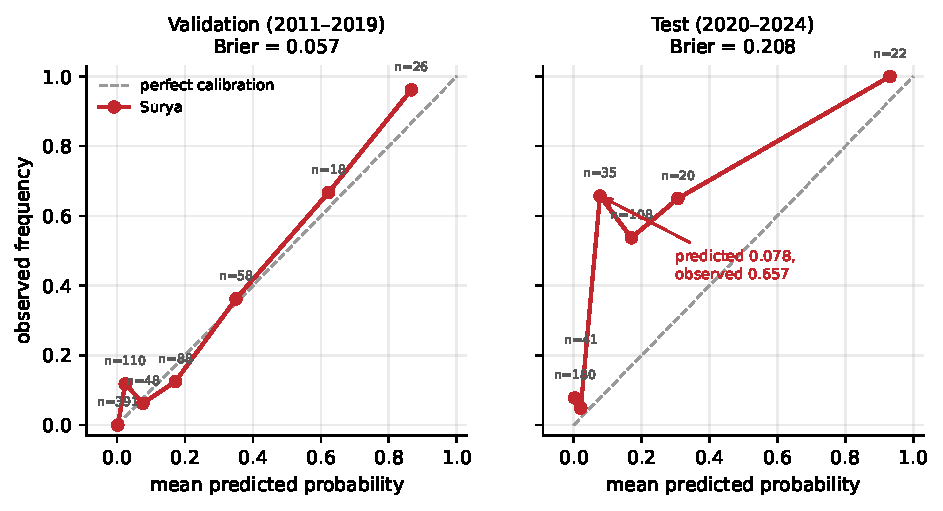
\includegraphics[width=\textwidth]{fig1_reliability}
\caption{Reliability diagrams. Calibration holds at solar minimum and collapses
at maximum; bin counts are annotated because several bins rest on very few
independent blocks.}
\end{figure}

\subsection{The common cause: base-rate non-stationarity}
\label{sec:baserate}

\begin{table}[htbp]
\centering
\caption{Per-year test statistics with the validation-frozen threshold.}
\begin{tabular}{lrrrr}
\toprule
year & $n$ & base rate & GOES logistic TSS & persistence TSS \\
\midrule
2020 & 8{,}784 & 0.0055 & 0.452 & $-0.005$ \\
2021 & 8{,}760 & 0.0613 & 0.514 & 0.270 \\
2022 & 8{,}760 & 0.2638 & 0.250 & 0.322 \\
2023 & 8{,}760 & 0.4435 & 0.056 & 0.293 \\
2024 & 8{,}784 & 0.6969 & 0.079 & 0.389 \\
\bottomrule
\end{tabular}
\end{table}

The positive rate rises 128-fold across the split ($0.0055 \rightarrow 0.6969$),
and the two methods respond in opposite directions: the frozen-threshold logistic
collapses from 0.514 in 2021 to 0.079 in 2024, while persistence climbs from
$-0.005$ to 0.389. Neither escapes the aggregation artefact, however. Pooled test
TSS is 0.554 for the logistic against a per-year range of 0.056--0.514, and 0.535
for persistence against a range of $-0.005$ to 0.389: for both, pooling
manufactures skill that no individual year shows.

\begin{figure}[htbp]
\centering
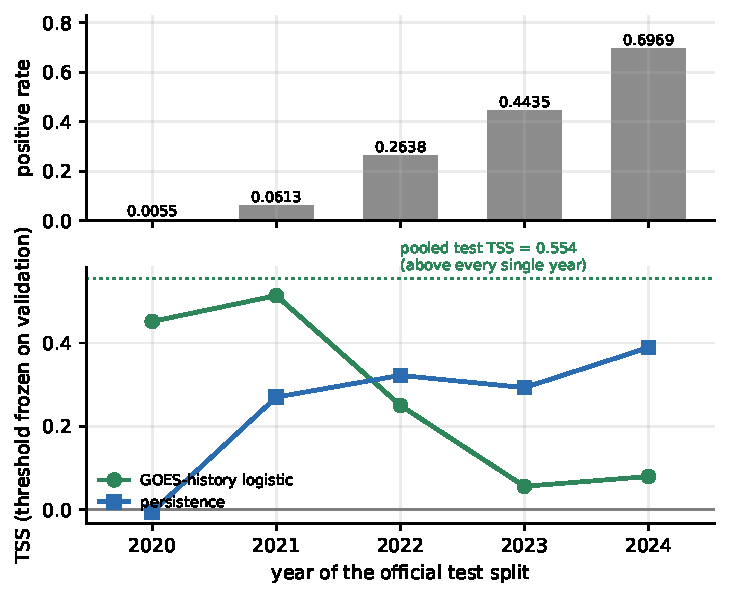
\includegraphics[width=0.75\textwidth]{fig2_base_rate_drift}
\caption{A 128-fold base-rate shift across the official test split breaks every
frozen threshold, and the pooled score sits above every individual year.}
\end{figure}

\section{Discussion}

\subsection{Without a cheap baseline, a modality's contribution is unmeasurable}

The question a flare benchmark should answer is not ``how well does this model
score?'' but ``what does solar imagery add over what we could already do?'' That
question is answerable only if the evaluation includes something that does not
use imagery. The reported comparison sets Surya against AlexNet and
ResNet50---both of which consume the same images, so every entry in the table
shares the modality under test, and the marginal value of imagery cancels out of
the comparison. Our results suggest that on this particular task the margin is
small or absent: a model with eleven coefficients and a single input channel
matches or exceeds it.

This should not be read as a verdict on the pretrained backbone. It is a verdict
on one binary downstream task, and a plausible reading is simply that 24-hour
M-class occurrence is largely determined by whether the Sun is \emph{already}
flaring---information fully contained in the X-ray record. If so, the task is a
poor instrument for measuring what a solar foundation model knows, and better
instruments exist: spatially resolved products, lead-time curves at longer
horizons, magnitude rather than occurrence, or transfer across the other
downstream tasks released with the model. Demonstrating value where cheap
features cannot reach would be a stronger claim than a marginal win where they
can.

\subsection{Non-stationary base rates make pooled scalar metrics misleading}

The solar cycle is the dominant nuisance variable in this problem, and the
official test split spans its steep rising phase. A 128-fold change in the
positive rate means that the 2020 task and the 2024 task are, statistically,
different problems that happen to share a label definition. Pooling them yields a
number (0.554) larger than any per-year value (0.056--0.514), a Simpson's
paradox produced not by a modelling error but by aggregation across a covariate
shift. Reporting that single number invites exactly the wrong inference.

The same mechanism explains the calibration result. A model whose probabilities
are faithful when flares are rare is systematically underconfident when they
become common, and the failure of Platt rescaling to transfer shows that this is
not a fixed bias but a function of the regime. Practically, this means any
deployed system must either re-calibrate online or condition explicitly on cycle
phase; a calibration certified during solar minimum is not evidence about solar
maximum.

We note that this pathology is not specific to heliophysics. Any rare-event
forecasting benchmark with a slow cyclic driver---seasonal epidemiology, wildfire
risk, certain financial regimes---will produce inflated pooled metrics and
non-transferable calibration if evaluated the same way. The fix is not more data
but stratified reporting.

\subsection{Complementarity is more useful than ranking}

Our regime split shows that the two predictors fail in disjoint places.
Persistence cannot, even in principle, anticipate an episode that has not begun,
and it necessarily false-alarms as an episode decays; those two statements are
definitional. In our sample the model covers part of that blind spot,
though---as Section~\ref{sec:onset} insists---on too few episodes to quote a
rate, and only at thresholds far below the one shipped. What can be defended
quantitatively is the pooled result: their disjunction outperforms both
components. For an operational user that is the actionable finding---not which
single forecaster is better on average, but that a trivial combination covers a
structural blind spot. It also suggests that benchmark tables listing models in
rank order obscure the more valuable information: \emph{where} each method's
skill lives.

\subsection{Uncertainty is not optional}

With 50 and 28 independent forecast blocks, and only 6 and 11 of them containing
any positive---95\% intervals span 0.46 to 0.81 TSS. Differences of 0.05--0.10
between methods, the differences that benchmark tables are usually built to
display, are therefore not resolvable at this sample size; across our ten
paired comparisons even the largest gap, 0.445, fails a family-wise correction
(Section~\ref{sec:power}). Reporting
point
estimates without intervals gives a false impression of resolution, and the
standard per-sample bootstrap makes this worse by ignoring within-block
autocorrelation and understating variance. Blocked resampling costs nothing and
should be routine.

\section{Recommendations}

\begin{enumerate}
\item Report climatology, persistence, and a statistical (non-imagery) baseline
alongside every deep model. This is not a new ask: NOAA SWPC verifies its own
flare forecasts against 30-day climatology and 1-day persistence
\citep{swpcverif}, and \citet{camporeale2025} recommend exactly this of research
models before they are ``claimed as an advance over current methods.''
\item State the evaluation split, years, and the threshold-selection procedure.
\item Report per-year or per-regime metrics; if pooled numbers are given, show
the stratified values beside them.
\item Report uncertainty using temporally blocked resampling, not per-sample
bootstrap, and quote the number of positive-containing blocks.
\item Publish reliability diagrams; treat calibration transfer across solar-cycle
phases as an explicit evaluation axis.
\item Keep the paper, the companion benchmark paper, the model card and the
dataset card consistent with one another and with the released files, and state
the event threshold numerically wherever it appears. Every discrepancy in
Section~\ref{sec:located} would have been caught by one pass reconciling the four
documents against the data.
\end{enumerate}

\section{Limitations}
\label{sec:limits}

\begin{itemize}
\item Model scoring uses a stratified 1{,}146-hour sample, not the full splits;
absolute values are sample-conditioned (mitigated by
Section~\ref{sec:sampling}'s sanity check).
\item The reliability tables condition on the model's stated probability, but
the sampling over-represents flare-active windows, which inflates the observed
frequency in every bin relative to the full splits. The validation--test
contrast is computed under the same sampling and survives it; absolute
statements such as ``close to faithful on validation'' are sample-conditioned,
and the sanity check of Section~\ref{sec:sampling} covers TSS, not calibration.
\item Both Surya's and the baseline's tuned thresholds in
Sections~\ref{sec:power}--\ref{sec:calib} are optimised in-sample, which flatters
both; Section~\ref{sec:cheap}'s full-split protocol freezes the threshold on
validation instead.
\item The full-split baseline numbers are \textbf{not matched} to our model
measurements; they corroborate but cannot substitute for the matched comparison
in Section~\ref{sec:cheap}.
\item Onset-level statements rest on 4 and 3 independent onset-containing blocks.
No onset rate---including the zero-catch observation---is estimable at this
effective sample size; Section~\ref{sec:onset} reports them descriptively for
that reason.
\item Even the headline scoreboard rests on 6 (validation) and 11 (test)
positive-containing blocks. Our own numbers inherit the limitation we document,
which is why every one of them is quoted with an interval.
\item Missing archive files cost about 15\% of the planned hours (125 of 864
validation, 73 of 480 test) and fragment some 24-hour windows into shorter runs.
Because we treat each recovered run as the resampling unit, this fragmentation is
reflected in the intervals rather than hidden by them; but it does mean our
blocks are not uniformly 24 hours long.
\item 196 of 74{,}760 training rows (0.26\%) were dropped for non-finite
features. These trace to four hours in the released record whose GOES class is
\code{A0.0}, giving a log-flux of $-\infty$ that propagates into up to seven
lagged features each.
\item Inference used bf16 autocast. We did not have GPU access for a
confirmatory fp32 run, so we bounded instead what one could change
(\code{precision\_sensitivity.py}). At the shipped 0.5 threshold \textbf{no hour
in either split lies within $10^{-3}$ of the decision boundary}, the closest are
0.0059 (validation) and 0.0039 (test) away, and an adversarial worst case in
which every hour within $10^{-2}$ flips the damaging way moves TSS by at most
0.002 and 0.008 respectively. At the tuned thresholds the same worst case moves
TSS by at most 0.033. Against intervals 0.46--0.81 wide these are immaterial. The
zero-catch observation of Section~\ref{sec:onset} is safer still: the largest
probability among the 27 test onset hours is 0.332, a margin of 0.168 below the
threshold. A confirmatory fp32 run remains desirable, but no conclusion here
depends on it.
\item A magnetogram-derived SHARP baseline was not run; the GOES-history model is
a weaker information set, which strengthens rather than weakens the argument.
\item Our persistence reference reads the complete hourly record rather than the
split file. This keeps three validation hours that a split-local lookup would
drop; the choice changes no reported score at three decimal places.
\end{itemize}

\section{Reproducibility}

\begin{sloppypar}
All probabilities, labels, code, and outputs are released. \code{heliofloor\_data.py}
is the canonical loader, metrics and block bootstrap, imported by everything else;
\code{heliofloor\_colab.py} regenerates the probabilities on a GPU;
\code{goes\_baseline.py} runs the matched comparison; \code{full\_split\_baseline.py}
the complete-split protocol; \code{analysis\_pack.py} the scoreboards, calibration,
transfer and regime split; \code{block\_support.py} the independent-block support
behind each claim; \code{onset\_ci.py} the onset rates and rule-of-three
correction; \code{paired\_diff.py} the paired method differences; \code{make\_figures.py} the four figures; and \code{verify\_paper.py}
recomputes every claim in this manuscript and prints a pass/fail line for each.
The three \code{probs\_*.csv} files carry the 1{,}146 scored hours.
\end{sloppypar}

Block plans regenerate identically from seed 42, and every bootstrap interval
reseeds per call so it reproduces independently of execution order. The scored
probabilities are committed, so all analysis reproduces on a CPU in minutes
with no GPU and no re-inference. Code and data:
\url{https://github.com/kadircanyildirm-crypto/heliofloor}.

\section*{Acknowledgements}

Analysis code and manuscript drafting were assisted by an AI coding
assistant. All results were produced by the released scripts, every
reported number is recomputed by \code{verify\_paper.py}, and the author
verified the label-leakage check, the split definitions and the quoted
comparison figures against primary sources.

\begin{thebibliography}{99}

\bibitem[Barnes et al.(2016)]{barnes2016}
Barnes, G., Leka, K.~D., Schrijver, C.~J., et al. 2016,
\emph{A Comparison of Flare Forecasting Methods. I. Results from the ``All-Clear'' Workshop},
The Astrophysical Journal, 829(2), 89.
\doi{10.3847/0004-637X/829/2/89}. arXiv:1608.06319.

\bibitem[Bloomfield et al.(2012)]{bloomfield2012}
Bloomfield, D.~S., Higgins, P.~A., McAteer, R.~T.~J., \& Gallagher, P.~T. 2012,
\emph{Toward Reliable Benchmarking of Solar Flare Forecasting Methods},
The Astrophysical Journal Letters, 747(2), L41.
\doi{10.1088/2041-8205/747/2/L41}. arXiv:1202.5995.

\bibitem[Bobra et al.(2014)]{bobra2014}
Bobra, M.~G., Sun, X., Hoeksema, J.~T., et al. 2014,
\emph{The Helioseismic and Magnetic Imager (HMI) Vector Magnetic Field Pipeline:
SHARPs -- Space-Weather HMI Active Region Patches},
Solar Physics, 289(9), 3549. \doi{10.1007/s11207-014-0529-3}. arXiv:1404.1879.

\bibitem[Bobra \& Couvidat(2015)]{bobra2015}
Bobra, M.~G., \& Couvidat, S. 2015,
\emph{Solar Flare Prediction Using SDO/HMI Vector Magnetic Field Data with a
Machine-learning Algorithm},
The Astrophysical Journal, 798(2), 135. \doi{10.1088/0004-637X/798/2/135}.
arXiv:1411.1405.

\bibitem[Campi et al.(2019)]{campi2019}
Campi, C., Benvenuto, F., Massone, A.~M., et al. 2019,
\emph{Feature Ranking of Active Region Source Properties in Solar Flare
Forecasting and the Uncompromised Stochasticity of Flare Occurrence},
The Astrophysical Journal, 883(2), 150. \doi{10.3847/1538-4357/ab3c26}.
arXiv:1906.12094.

\bibitem[Camporeale \& Berger(2025)]{camporeale2025}
Camporeale, E., \& Berger, T.~E. 2025,
\emph{Verification of the NOAA Space Weather Prediction Center Solar Flare
Forecast (1998--2024)},
Space Weather, 23(10), e2025SW004546. \doi{10.1029/2025SW004546}.
arXiv:2508.01114.

\bibitem[Leka et al.(2019a)]{leka2019b}
Leka, K.~D., Park, S.-H., Kusano, K., et al. 2019a,
\emph{A Comparison of Flare Forecasting Methods. II. Benchmarks, Metrics, and
Performance Results for Operational Solar Flare Forecasting Systems},
The Astrophysical Journal Supplement Series, 243(2), 36.
\doi{10.3847/1538-4365/ab2e12}. arXiv:1907.02905.

\bibitem[Leka et al.(2019b)]{leka2019c}
Leka, K.~D., Park, S.-H., Kusano, K., et al. 2019b,
\emph{A Comparison of Flare Forecasting Methods. III. Systematic Behaviors of
Operational Solar Flare Forecasting Systems},
The Astrophysical Journal, 881(2), 101.
\doi{10.3847/1538-4357/ab2e11}. arXiv:1907.02909.

\bibitem[Nishizuka et al.(2017)]{nishizuka2017}
Nishizuka, N., Sugiura, K., Kubo, Y., et al. 2017,
\emph{Solar Flare Prediction Model with Three Machine-learning Algorithms using
Ultraviolet Brightening and Vector Magnetograms},
The Astrophysical Journal, 835(2), 156. \doi{10.3847/1538-4357/835/2/156}.
arXiv:1611.01791.

\bibitem[NOAA SWPC(n.d.)]{swpcverif}
NOAA Space Weather Prediction Center,
\emph{Solar Activity Forecast Verification} (M-class and X-class flare
probability verification, 1986--2013).
\url{https://www.spaceweather.gov/content/solar-activity-forecast-verification}
(accessed 2026-08-27).

\bibitem[Park et al.(2020)]{park2020}
Park, S.-H., Leka, K.~D., Kusano, K., et al. 2020,
\emph{A Comparison of Flare Forecasting Methods. IV. Evaluating Consecutive-day
Forecasting Patterns},
The Astrophysical Journal, 890(2), 124.
\doi{10.3847/1538-4357/ab65f0}. arXiv:2001.02808.

\bibitem[Roy et al.(2025)]{roy2025}
Roy, S., Schmude, J., Lal, R., et al. 2025,
\emph{Surya: Foundation Model for Heliophysics}, arXiv:2508.14112.
Model weights: \code{nasa-ibm-ai4science/Surya-1.0} and
\code{nasa-ibm-ai4science/solar\_flares\_surya}, Hugging Face, Apache 2.0.

\bibitem[Roy et al.(2026)]{roy2026}
Roy, S., Hegde, D.~V., Schmude, J., et al. 2026,
\emph{SuryaBench: Benchmark Dataset for Advancing Machine Learning in
Heliophysics and Space Weather Prediction},
Scientific Data, 13(1), 712. \doi{10.1038/s41597-026-06552-5}.
Preprint arXiv:2508.14107. Flare task data:
\code{nasa-ibm-ai4science/surya-bench-flare-forecasting}, Hugging Face, CC BY 4.0.

\bibitem[van der Sande et al.(2023)]{vandersande2023}
van der Sande, K., Mu\~{n}oz-Jaramillo, A., \& Chatterjee, S. 2023,
\emph{Probabilistic Solar Flare Forecasting Using Historical Magnetogram Data},
The Astrophysical Journal, 955(2), 148. \doi{10.3847/1538-4357/acf49a}.
arXiv:2308.15410.

\end{thebibliography}

\end{document}
